% -----------------------------------------------
% Template for ISMIR 2014
% (based on earlier ISMIR templates)
% -----------------------------------------------

\documentclass{article}

\usepackage{ismir2014,amsmath,cite,url,graphicx}
\usepackage[utf8]{inputenc}

\title{Spotify-ed: Music Recommendation and Discovery in Spotify}

% Single address
% To use with only one author or several with the same address
% ---------------
%\oneauthor
% {José Bateira}
% {Affiliations should be omitted for double-blind reviewing}

% Two addresses
% --------------
%\twoauthors
%  {José Bateira} {School \\ Department}
%  {Second author} {Company \\ Address}

% Three addresses
% --------------
% \threeauthors
%   {José Bateira} {Porto, Portugal \\ {\tt ei10133@fe.up.pt}}
%   {Second author} {\bf Retain these fake authors in\\\bf submission to preserve the formatting}
%   {Third author} {Affiliation3 \\ {\tt author3@ismir.edu}}

% Four addresses
% --------------
\fourauthors
 {José Bateira} {DEI-FEUP/INESC TEC \\ {\tt ei10133@fe.up.pt}}
 {Fabien Gouyon}{INESC TEC \\ {\tt fgouyon@inescporto.pt}}
 {Matthew Davies} {INESC TEC \\ {\tt mdavies@inescporto.pt}}
 {Marcelo Caetano} {INESC TEC \\ {\tt mcaetano@inescporto.pt}}

\begin{document}
%
\maketitle
%
\begin{abstract}
  This demo presents the Spotify App\footnote{\url{https://developer.spotify.com/technologies/apps}} of RAMA\footnote{\url{http://rama.inescporto.pt}} that aims to improve the way music recommendations are shown in Spotify\footnote{\url{http://spotify.com}}.
  This version implements most of the current features of RAMA's original website\footnote{\url{http://rama.inescporto.pt/app}}: edition of the visualization parameters (to obtain more detailed graphs), edition of the graph by adding and removing node artists (for users that want to meticulously edit the graph) and visualization of the tags/genres that describe an artist in the graph.
  The metadata used throughout the application is provided by Spotify's and Echonest's API\footnote{\url{http://developer.echonest.com}}.

\end{abstract}

  \section{Music Discovery Tools in Spotify} % (fold)
  \label{sec:spotify_tools}
  
    The recommendation systems in Spotify present the suggestions to the users in the form of lists and/or grids.
    This is not ideal since the user cannot understand the reason behind such recommendations.

    Spotify provides a set of tools for the users to discover new music.
    Some are tailored for the user, while others show what bands are more popular at the moment.
    The tools are: Browse, Activity, Discovery, Radio and Spotify Apps.
    The latter is a different possibility for the user to discover new music.
    It relies on Spotify apps that other services have developed, for example, Last.fm\footnote{\url{http://last.fm}} developed their application that uses its recommendation system. 
    This way, Spotify users can have the best of both worlds from Spotify and Last.fm all in one application.
    But the way the recommendations are displayed (lists and grids) remains an issue.

  % section spotify_tools (end)

  \section{RAMA in Spotify} % (fold)
  \label{sec:rama}
  
  RAMA breaks the pattern by introducing a visual representation of a network of music artists.
  There are other approaches that solve this problem in a similar manner (for example, \url{http://liveplasma.com} and \url{http://musicroamer.com}).
  Most of these applications use Youtube\footnote{\url{http://youtube.com}} to stream the music tracks.
  This is not ideal given that: the sound quality is not appropriate for music streaming; Youtube is not a music oriented service and the \emph{noise} it exposes makes it an unreliable source for music stream.
  Spotify can tackle those issues given its large music catalogue and high quality stream.

  Among all the possibilities that Spotify has made available for developers\footnote{\url{http://developer.spotify.com}}, Spotify Apps is the ideal choice: by implementing RAMA's concept into a Spotify App, the Spotify user gets a brand new tool to explore new music in a more natural and intuitive way \emph{inside} Spotify itself.

  \section{Main Features} % (fold)
  \label{sec:features}
  
    \subsection{Visualization of the Artists' Map} % (fold)
    \label{sub:visualization}

      RAMA's Spotify App automatically draws the map with the current playing artist as the main node, as seen in Figure~\ref{fig:spotify_app}.
      \begin{figure}[hb]
        \begin{center}
          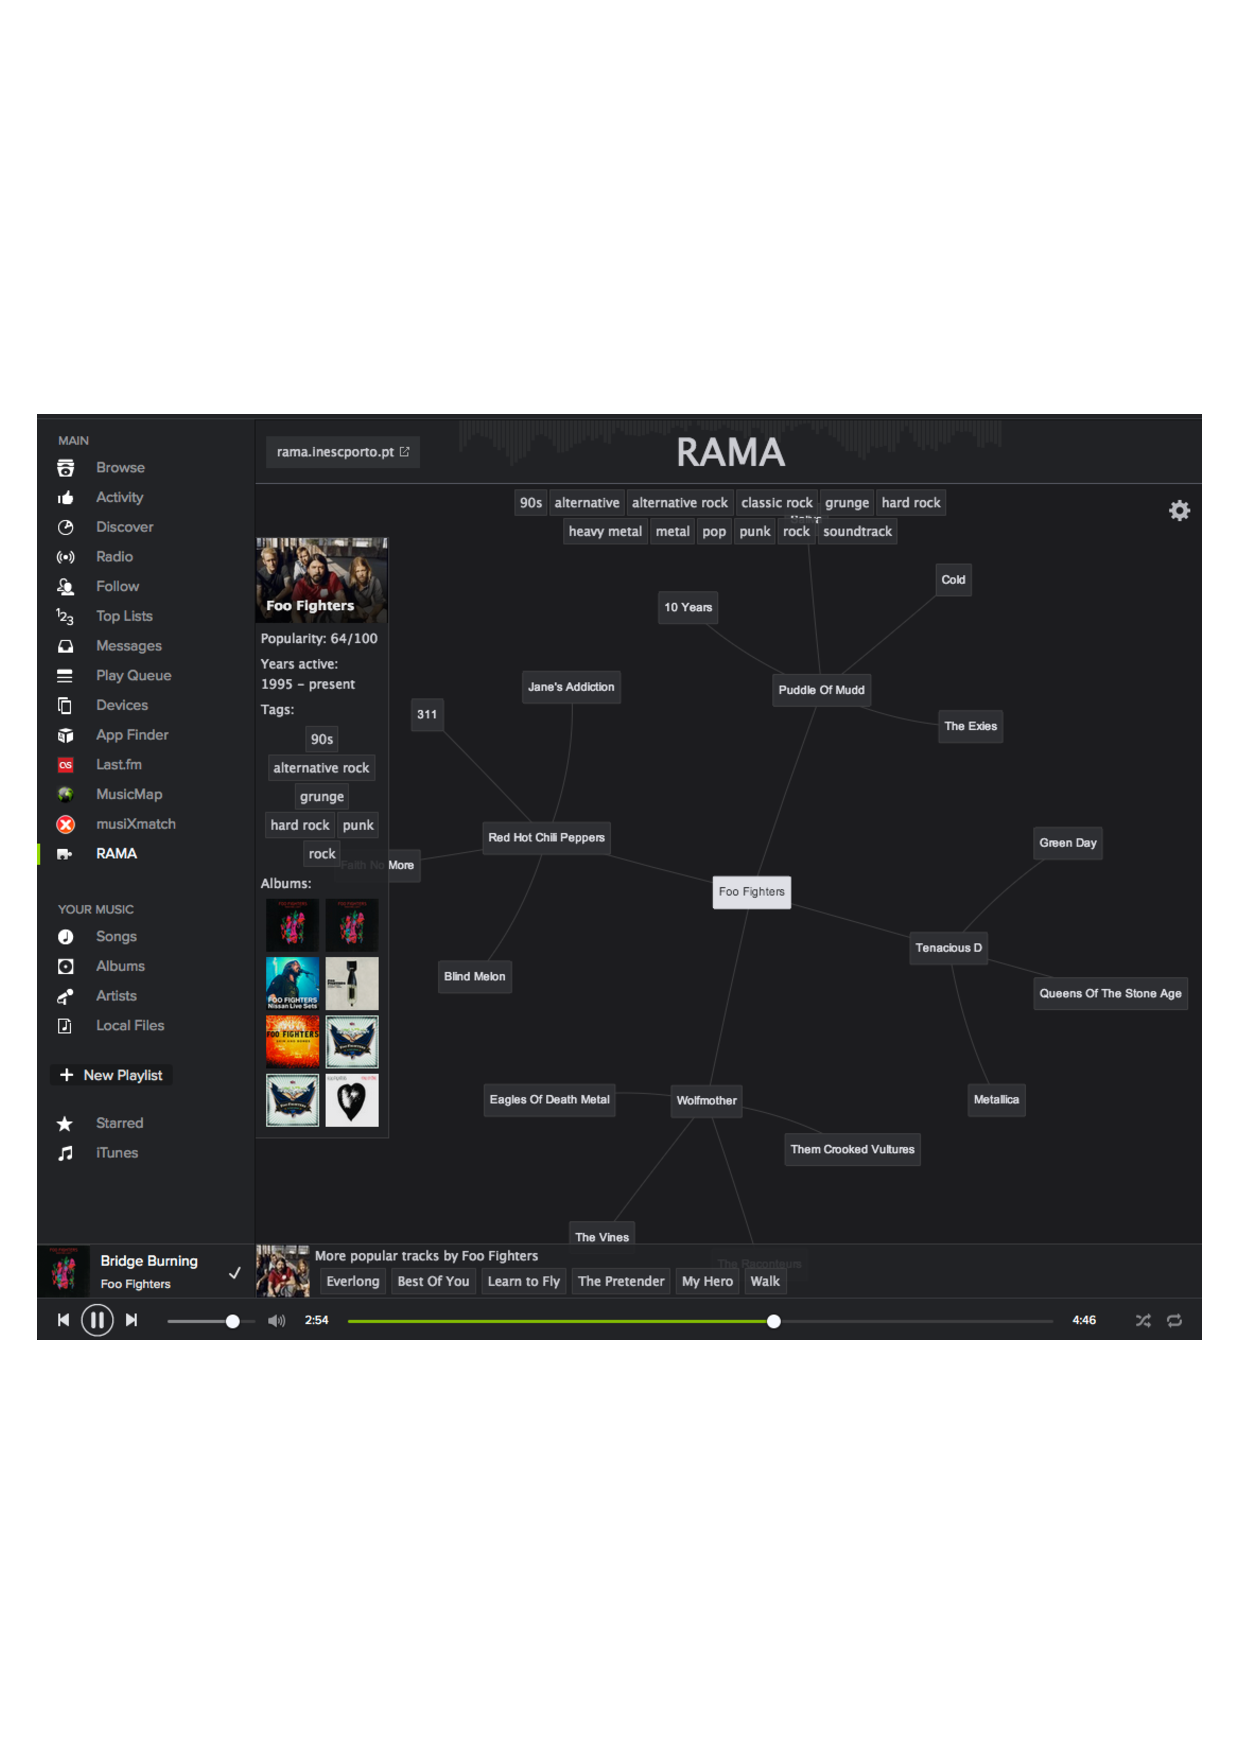
\includegraphics[width=\columnwidth]{../report/figures/graph_rootnode.pdf}
        \end{center}
        \caption{RAMA Spotify App opened inside the Spotify Desktop Client}
        \label{fig:spotify_app}
      \end{figure}
      The graph-like structure is created by recursively fetching a list of related artists from each artist using Spotify's API\footnote{\url{https://developer.spotify.com/docs/apps/api/1.0/api-models-artist.html}}.

    \subsection{Visualization Parameters} % (fold)
    \label{sub:visualization_parameters}

      The visualization parameters can be personalized by the user in the settings menu in order to create richer graphs that match the user's preferences better.
      The depth value of a graph determines how deep the recursive algorithm goes when constructing the graph, meaning, depth is the maximum distance between the root node and any other node in the graph.
      The branching value of a tree graph determines the maximum number of child nodes a node can have.
      The tree mode option indicates whether the graph to be built is a tree graph or not.
      This means that when the tree mode is on, the graph has less edges (which leaves the graph more clean) and so it becomes a tree graph.

    \subsection{Graph Edition} % (fold)
    \label{sub:graph_edition}
      
      The available features to edit the graph are: expand node, delete node and create a new map. These interactions are available in the Artist Menu (Figure~\ref{fig:artist_menu}).
      The expand node action allows the user to expand a node further (ignoring the graph’s branching value).
      The delete node action allows the user to delete a node from the graph.
      These two actions are useful for when the user wants to construct the graph to his/her needs.
      The new map action lets the user create a whole new graph from a another node. This way the root node will be the selected node of the new graph.

    \subsection{Artist Menu} % (fold)
    \label{sub:artist_menu}
    
      The user is able to see additional information about artists in the Artist Menu (Figure~\ref{fig:artist_menu}) such as its popularity value, albums and tags, as well as perform the expand and new map functions described in \ref{sub:graph_edition}.
      \begin{figure}[th]
        \begin{center}
          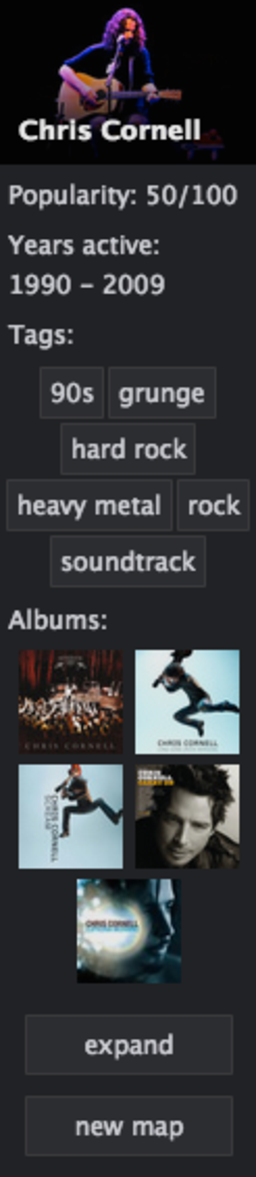
\includegraphics[width=0.2\columnwidth]{../report/figures/artist_menu.pdf}
        \end{center}
        \caption{Artist Menu with information about “Chris Cornell”}
        \label{fig:artist_menu}
      \end{figure}
      When the user selects a node by clicking on it, the artist menu updates the displayed information.
      The popularity, the albums and the tags are metadata information retrieved from Spotify’s API, although Echonest’s API is also used as a fallback source for the tags (sometimes Spotify’s API responds with a small number of results).

    \subsection{Tags Overlay} % (fold)
    \label{sub:tags_overlay}
    
      The tags overlay menu (Figure~\ref{fig:tags_overlay}) is meant to enhance the user’s understanding on the displayed artists’ nodes regarding their tags. These tags are the same ones used in the Artist Menu (Figure~\ref{fig:artist_menu}).
      \begin{figure}[th]
        \begin{center}
          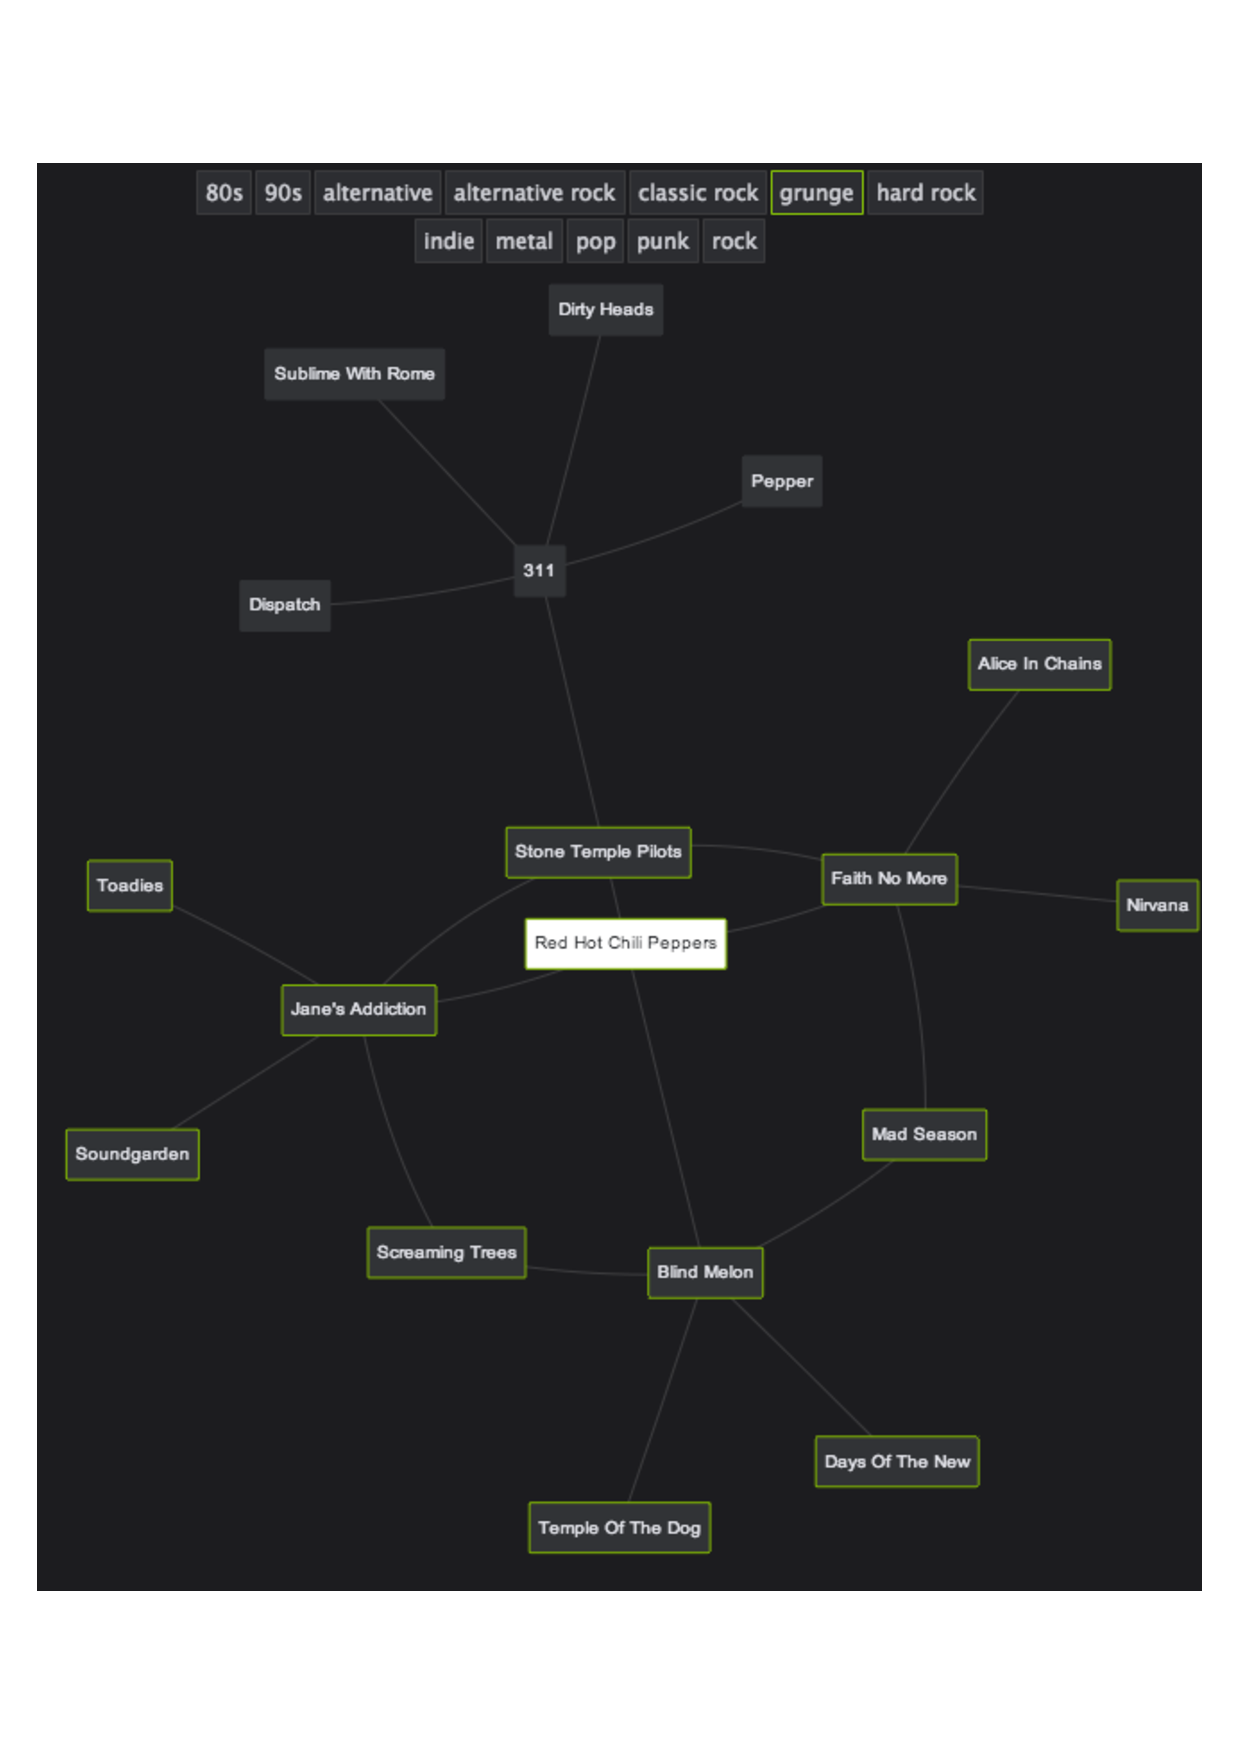
\includegraphics[width=\columnwidth]{../report/figures/tags_overlay.pdf}
        \end{center}
        \caption{Tags Overlay}
        \label{fig:tags_overlay}
      \end{figure}
      They are selectable, and so, when clicked, the respective artist nodes that are described by those tags, are highlighted (as seen in Figure~\ref{fig:tags_overlay}).
      The tags shown in this menu, are just a small sample of the artists’ tags of the whole graph.



% \begin{thebibliography}{citations}

% \bibitem {Author:00}
% E. Author:
% ``The Title of the Conference Paper,''
% {\it Proceedings of the International Symposium
% on Music Information Retrieval}, pp.~000--111, 2000.

% \bibitem{Someone:10}
% A. Someone, B. Someone, and C. Someone:
% ``The Title of the Journal Paper,''
% {\it Journal of New Music Research},
% Vol.~A, No.~B, pp.~111--222, 2010.

% \bibitem{Someone:04} X. Someone and Y. Someone: {\it Title of the Book},
%     Editorial Acme, Porto, 2012.

% \end{thebibliography}

% \bibliography{../report/bib/myrefs}
\bibliographystyle{unstrnat}

\end{document}
